\documentclass[11pt]{article}

\usepackage[a4paper,margin=1in]{geometry}
\usepackage{amsmath}
\usepackage{amssymb}
\usepackage{booktabs}
\usepackage{float}
\usepackage{graphicx}
\usepackage{pdflscape}
\usepackage{tabularx}
\usepackage{tikz}
\usetikzlibrary{arrows.meta,positioning}
\usepackage[hidelinks]{hyperref}
\usepackage[authoryear,round]{natbib}
\usepackage{siunitx}
\sisetup{group-separator={,},group-minimum-digits=4}

\newcommand{\Hnorm}{1-H_{\mathrm{norm}}}

\title{Controlled Evaluation of Class-Imbalance Mitigation\\
Across Histopathology Patch Classification and WSI-Level MIL}
\author{Yannik Queisler}
\date{\today}

\begin{document}
\maketitle

\begin{abstract}
\begingroup
\setlength{\emergencystretch}{2em}
\noindent This study evaluates methods for mitigating class imbalance in computational pathology, covering patch classification and whole-slide multiple-instance learning (MIL) in CAMELYON16, TCGA-UT, BRACS, and PANDA, all represented with frozen Virchow2 features. Patient- or case-disjoint splits are created before imbalance is manipulated, and only training support changes: a full natural anchor is accompanied by size-matched balanced, moderate ($\rho=10$), and severe ($\rho=100$ where feasible) conditions. Validation and test split units, held-out prevalence, training-set size, model family, and numbers of optimizer updates remain fixed. Patch conditions retain a common patient/case and slide pool while changing patch allocation; MIL conditions vary slide support and report the resulting change in independent-unit diversity. The primary discrimination endpoint is balanced accuracy, evaluated alongside a co-primary tail-calibration endpoint. Mitigation recovery is assessed only when prespecified thresholds show a meaningful imbalance-induced deficit on the corresponding endpoint. Secondary analyses address classwise discrimination, tail-sensitive calibration, computational cost, intrinsic separability, and condition-specific learnability.
\par
\endgroup
\end{abstract}

\setcounter{tocdepth}{2}
\tableofcontents
\clearpage

\section{Introduction}
Class imbalance changes the empirical objective faced by a classifier: frequent classes supply more optimization terms, while rare classes may contribute too little evidence to establish stable decision boundaries. In pathology, the problem occurs at two distinct prediction units. Patch classification uses directly labelled crops, whereas WSI-level MIL predicts from bags whose instances inherit only a weak slide label. The same slide cohort can therefore be nearly balanced between diagnoses while containing very sparse class-informative tissue. Aggregate accuracy does not isolate either failure mode, motivating class-balanced discrimination and probability-quality evaluation \citep{saini2023tacklingClass,zhang2023deepLong,mosquera2024classImbalance}.

Native-dataset comparisons do not identify an imbalance effect by themselves. They simultaneously vary task, class separability, training support, label granularity, and evaluation prevalence. This study instead changes class allocation only in the training partition and retains identical natural validation and test cohorts. A size-matched balanced CE condition estimates attainable performance at the same training budget, so mitigation can be interpreted as recovery of damage attributable to the imposed imbalance rather than as an unconstrained gain over a convenient baseline.

The study addresses three research questions:
\begin{description}
  \item[RQ1.] \textbf{Effect of imbalance.} At fixed task, split-unit partition, encoder, training-set size, and evaluation set, how does increasing training imbalance affect tail-class discrimination and calibration in patch classification and WSI-level MIL?
  \item[RQ2.] \textbf{Mitigation effectiveness.} Which mitigation methods recover performance lost specifically to training imbalance, and what are their calibration and computational costs?
  \item[RQ3.] \textbf{Predictors of damage and mitigation headroom.} Can small exploratory models help explain why some controlled comparisons are more vulnerable than others? Specifically, are imbalance severity and intrinsic separability associated with whether damage occurs, how large it is, and how much is recovered after damage? Condition-specific learnability and independent support are examined as sensitivity predictors.
\end{description}
RQ1 establishes whether a recoverable problem exists, and RQ2 asks which methods address that demonstrated deficit. RQ3 is an exploratory association analysis rather than another method ranking: it relates prespecified properties of each comparison to damage occurrence, damage magnitude, and, where damage is demonstrated, recovery. The datasets and preprocessing provenance are documented in the companion dataset report, and all detailed method objectives and variants are defined in the companion methods report \citep{queisler2026datasets,queisler2026imbalanceMethods}.

\section{Experimental Design}
\label{sec:design}
A controlled imbalance experiment is informative only when the balanced and imbalanced models differ in their training class allocation rather than in their data source, representation, or evaluation cohort. The design therefore establishes the split-unit partition, frozen features, and held-out examples once, then constructs several training distributions at a common support budget. The following subsections define the two prediction regimes, explain how their evidence is controlled, and specify how mitigation methods are trained and compared.

Readers seeking a compact visual entry point can consult the benchmark overview in Appendix~\ref{app:overview} (Figure~\ref{fig:benchmark-overview}); the subsections below provide the formal specification.

\subsection{Datasets and prediction regimes}
\label{sec:data}
Table~\ref{tab:datasets} defines the prediction example and label in each available dataset--regime. The terms \emph{patch} and \emph{tile} both denote a $256\times256$ image crop; \emph{patch} is used throughout this report. A patch-level example is one such crop with the label specified in the second column. A bag-level example is one WSI represented by frozen embeddings of its eligible patches and receives one label for the entire WSI.

Every eligible patch embedding enters the MIL model for its WSI, so bag size reflects the tissue that remains after the dataset-specific eligibility pipeline. The complete bag for a given slide is identical across training conditions and methods.

Before examples are selected, each \emph{split unit}---a patient or participant where available and a biopsy/WSI otherwise---is assigned to exactly one partition: the training, validation, or test cohort. All slides from the same split unit follow that assignment. Dataset--regime eligibility is also fixed before splitting. A sample is excluded if it lacks a valid target or split-unit identifier, yields no patch under the dataset-specific tissue rule, lacks an annotation required to assign a patch label, or lacks readable frozen features. The same rules are applied before constructing every imbalance condition.

\begin{table}[ht]
  \centering
  \scriptsize
  \begin{tabularx}{\linewidth}{@{}l>{\raggedright\arraybackslash}X>{\raggedright\arraybackslash}X>{\raggedright\arraybackslash}X@{}}
    \toprule
    Dataset & Patch-level example and label & MIL bag and bag label & Split unit \\
    \midrule
    CAMELYON16 & Non-overlapping tissue crop at \num{20}x; tumor if at least \num{50}\% of its aligned mask cell is tumor, normal otherwise & One WSI bag; metastasis-bearing (tumor) versus normal slide & Slide (one slide per patient) \\
    TCGA-UT & Author-supplied tumor-region crop; inherits its source WSI's cancer type & One diagnostic-WSI bag; the same one of \num{32} cancer types & TCGA participant \\
    BRACS & Non-overlapping crop from a pathologist-annotated ROI; inherits one of seven ROI subtypes & One WSI bag; official seven-class WSI label defined by the most aggressive lesion detected in the slide & Patient \\
    PANDA & Foreground crop; cancer if at least \num{50}\% of its aligned provider-specific mask cell is cancer, benign otherwise & One biopsy-WSI bag; ordinal ISUP grade \num{0}--\num{5} & Biopsy (one WSI) \\
    \bottomrule
  \end{tabularx}
  \caption{Dataset-specific definitions of patch-level examples and bag-level examples. Only TCGA-UT uses the same target in both regimes. CAMELYON16 and PANDA change diagnostic granularity, while BRACS changes from the annotated ROI subtype to the official most-aggressive-lesion WSI subtype.}
  \label{tab:datasets}
\end{table}

\paragraph{Patch classification.}
Eligible patches are embedded once with frozen Virchow2. Concatenating the CLS token and mean patch token gives 2560 input features \citep{vorontsov2024virchow,zimmermann2024virchow2}. For CAMELYON16 and PANDA, a patch label is derived from the spatially aligned expert mask and can differ from the WSI label. A TCGA-UT patch inherits the cancer-type label of the diagnostic WSI from which the dataset authors cropped it. A BRACS patch inherits the subtype of its pathologist-annotated ROI. All patches that pass these dataset-specific eligibility and label rules enter the eligible pool before condition-specific training subsampling. The common classifier is a two-layer multilayer perceptron (MLP) with a 512-unit hidden representation, rectified linear unit (ReLU) activation, dropout, and a linear class output. CFAL alone replaces the linear output with a prototype-based affinity head; OKO adds a training-only auxiliary head that is discarded for evaluation.

\paragraph{WSI-level MIL.}
A slide is one bag of frozen patch embeddings; here, an \emph{instance} means one patch representation inside that bag, not a separately labelled training example. CAMELYON16 bags use the slide diagnosis, TCGA-UT bags use the diagnostic WSI's cancer type, and PANDA bags use the biopsy's ordinal ISUP grade. A BRACS bag uses the official seven-class WSI annotation, which the dataset defines from the most aggressive lesion detected in the slide. This label is read from the official WSI metadata rather than reconstructed from ROI annotations, so WSIs without released ROIs remain eligible and no project-specific severity ordering can alter the target. BRACS WSIs are sampled at \num{20}x into non-overlapping $256\times256$ patches and use the CAMELYON16 foreground stack: at least \num{10}\% Otsu foreground, grayscale standard deviation of at least \num{8}, Canny edge evidence, and at least two tissue neighbours. The common attention-MIL model maps every eligible instance to a 256-dimensional space, assigns normalized attention weights, and classifies their weighted average. SC-MIL adds a training projection head for its contrastive objective, and MDE-inspired MIL replaces the single classifier with two expert heads. Slide labels are the only supervision; patch labels, ROI labels, and masks are not used by the primary MIL training runs \citep{brancati2022bracs,queisler2026datasets}.

\paragraph{Comparative scope.}
Only TCGA-UT permits a direct patch-versus-WSI comparison. Both regimes predict the same cancer-type label within the same participant-disjoint cohort. In CAMELYON16, patch classification detects tumor tissue, whereas a WSI bag is classified as metastasis-bearing or normal. In PANDA, patch classification detects cancer tissue, whereas a WSI bag predicts the biopsy's ISUP grade. In BRACS, a patch predicts its ROI-specific subtype, whereas a WSI bag predicts the official most-aggressive-lesion subtype for the complete slide. The CAMELYON16, PANDA, and BRACS regimes are therefore separate dataset--target groups rather than paired measurements of one task.

\subsection{Controlled comparison}
The construction asks a simple counterfactual question: how would the same prediction task perform if a fixed training budget were distributed evenly across classes rather than concentrated in a head class? Answering this question requires more than specifying an imbalance ratio. The comparison must first fix the split-unit partition, eligible examples, representation, evaluation cohort, and total controlled training support; only then can class allocation be changed. Figure~\ref{fig:controlled-construction} summarizes this separation between fixed design choices and the intended intervention.

\begin{figure}[ht]
  \centering
  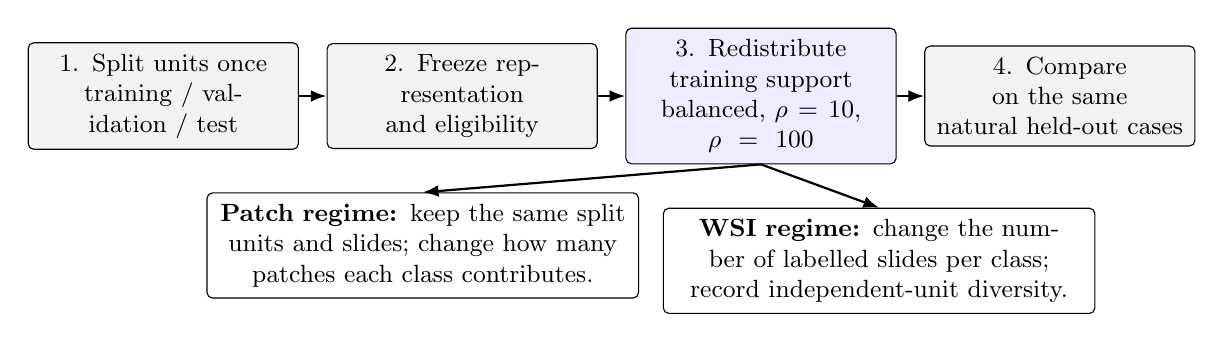
\begin{tikzpicture}[
    box/.style={draw, rounded corners=2pt, align=center, inner sep=4pt, font=\small, text width=3.15cm, minimum height=1.15cm},
    fixed/.style={box, fill=gray!10},
    varied/.style={box, fill=blue!7},
    note/.style={box, fill=white, text width=5.2cm, minimum height=1.0cm},
    arrow/.style={-{Latex[length=2mm]}, thick}
  ]
    \node[fixed] (split) {1. Split units once\\training / validation / test};
    \node[fixed, right=0.35cm of split] (freeze) {2. Freeze representation\\and eligibility};
    \node[varied, right=0.35cm of freeze] (construct) {3. Redistribute training support\\balanced, $\rho=10$, $\rho=100$};
    \node[fixed, right=0.35cm of construct] (evaluate) {4. Compare on the same\\natural held-out cases};
    \node[note, below=0.55cm of freeze, xshift=-0.5cm] (patch) {\textbf{Patch regime:} keep the same split units and slides; change how many patches each class contributes.};
    \node[note, below=0.55cm of construct, xshift=1.5cm] (wsi) {\textbf{WSI regime:} change the number of labelled slides per class; record independent-unit diversity.};
    \draw[arrow] (split) -- (freeze);
    \draw[arrow] (freeze) -- (construct);
    \draw[arrow] (construct) -- (evaluate);
    \draw[arrow] (construct.south) -- (patch.north);
    \draw[arrow] (construct.south) -- (wsi.north);
  \end{tikzpicture}
  \caption{Controlled construction of the benchmark. Gray steps are fixed within a split; the blue step is the intended intervention. Patch imbalance redistributes patches within a common split-unit and slide pool, whereas WSI imbalance changes labelled slide support.}
  \label{fig:controlled-construction}
\end{figure}

\noindent Each eligible dataset--regime--split has four training conditions:
\begin{enumerate}
  \item the full natural training set, used only as a descriptive anchor;
  \item a size-matched balanced training set;
  \item a moderate imbalance condition targeting $\rho=10$; and
  \item a severe imbalance condition targeting $\rho=100$ where feasible.
\end{enumerate}
The balanced, moderate, and severe conditions contain the same total training support $T$: patches for patch classification and slides for MIL. The shared $T$ is selected jointly with severity, not from size alone: for each requested ratio, construction first finds the largest ratio the training data can realize at any candidate $T$, then fixes $T$ to the largest value attaining those maxima simultaneously for every locked tail assignment, subject to the support constraints defined below. A larger $T$ chosen without regard to severity can flatten the realized profile toward the balanced condition even when a smaller $T$ would have supported the intended contrast, which would defeat the comparison the three conditions exist to make. The natural anchor may contain a different total and is excluded from the imbalance deficit and recovery estimands in Section~\ref{sec:recovery}. Thus contrasts among the three controlled conditions change class allocation without also changing the number of training examples.

The target ratio $\rho_{\mathrm{target}}\in\{1,10,100\}$ specifies the intended intervention, but integer allocation and finite inventories can change the realized class distribution. The achieved ratio is therefore recomputed from every manifest. For realized class supports $N_1,\ldots,N_K$, it is
\begin{equation}
  \rho_{\mathrm{achieved}}=\frac{N_{\max}}{N_{\min}}.
  \label{eq:rho}
\end{equation}
This quantity records the extreme head--tail contrast. The complementary normalized-entropy deficit
\begin{equation}
  \Hnorm=1-\frac{-\sum_{c=1}^{K}p_c\log p_c}{\log K},
  \qquad p_c=\frac{N_c}{\sum_jN_j}.
  \label{eq:entropy}
\end{equation}
\noindent uses all classes and is normalized for class count: it is zero for a balanced allocation and increases as support becomes concentrated. Both quantities are computed separately at patch and slide level from each realized training manifest. Per-class split-unit, slide, and patch counts are reported alongside them, because neither scalar reveals whether many patches originate from only a few cases.

Split-unit-disjoint training, natural-validation, and natural-test partitions are created first. Imbalance manipulation is confined to training support. Within a split, every condition uses exactly the same validation and test cases and eligible held-out examples. No held-out example is deleted, duplicated, or reweighted according to the training severity. Patch-level evaluation uses every eligible held-out patch, and slide-level evaluation uses every eligible held-out slide. Consequently, recall is estimated from all available held-out cases and prevalence-dependent precision and macro F1 are compared at one fixed test prevalence.

The validation cohort also retains its natural distribution. It is used for hyperparameter and checkpoint selection but never resized to resemble a training condition. Training, validation, and test manifests are versioned with split-unit identifiers, class counts, construction seed, and content hashes before model fitting.

\subsection{Independent evidence and support floors}
A patch is a training example, but it is not independent evidence when thousands of patches come from the same case or slide. In this report, \emph{independent support} therefore means the number of distinct split units and slides that underlie a class's training examples. Controlling this support prevents an apparent patch-level head--tail contrast from being merely a contrast between many correlated crops from one case and fewer crops from another.

The rule is adapted to the prediction regime. For patch classification, a fixed per-class split-unit pool and, within it, a fixed slide pool are made available to the balanced and all imbalanced conditions: every condition draws its patches only from this pool, and the condition with the largest patch allocation for a class covers the pool in full, so no unit in it goes unused by every condition together. A smaller condition for the same class, in particular a severe tail count well below that maximum, may leave some pool units untouched; this is the intended shape of an imbalanced allocation, not a violation of the shared pool. Sampling visits split units, then slides within units, and only then patches. No split unit may supply more than 10\% of a class's patch allocation and no slide more than 5\%; deterministic round-robin selection enforces these caps before any unit is revisited. Patch imbalance can therefore change the number of patches per class without changing which split-unit and slide pools are available to draw from. For MIL, a slide is itself the labelled example, so reducing slide support necessarily reduces independent support. Selection visits split units before taking additional slides from the same unit; each slide contributes once, and no unit supplies more than 10\% of a class's slides. MIL contrasts are consequently interpreted as controlled slide-support imbalance, including its induced change in independent-unit diversity. Every manifest reports per-class split-unit, slide, and patch counts, maximum contributions, and the fraction of the eligible independent pool retained.

The smallest defensible tail support is estimated before the definitive comparison with a \emph{support pilot}. These balanced CE runs ask when additional independent training units cease to materially improve natural-validation performance; they do not tune a hyperparameter or contribute observations to the definitive analysis. In the patch regime, one pilot unit is a split unit, or a slide where split unit and slide coincide. Each selected unit contributes the same fixed quota $q_{\mathrm{patch}}$ of patches, distributed as evenly as possible over its eligible slides. The quota is the largest value the patient and slide contribution caps admit at every candidate level and every construction ordering, held fixed so increasing a pilot level adds independent units rather than patches per unit. A caps-admissible quota is necessary but not sufficient: a unit cannot supply more patches than it holds, so a unit is eligible for a candidate level only if its own inventory meets the candidate quota, and the quota at a given level is set from that level's order statistic of per-unit inventory over the eligible units rather than from the scarcest unit in one seeded ordering. A candidate level that no quota can satisfy is dropped from the curve rather than reusing a looser quota from a larger level. In the MIL regime, one pilot unit is a labelled slide represented by all its eligible instances.

Nested pilots compare $10,15,20,30,$ and $50$ units per class, or all available units when the scarcest class has fewer. They are repeated for three independently seeded \emph{construction orderings}. An ordering is a fixed sequence of eligible units; its prefix of length $m$ is simply the first $m$ units in that sequence. Thus the 15-unit pilot retains the same first 10 units as the 10-unit pilot and adds the next five. At lower levels of the hierarchy, every split unit has a fixed slide order and every slide has a fixed patch order. Figure~\ref{fig:construction-hierarchy} illustrates this nesting.

\begin{figure}[ht]
  \centering
  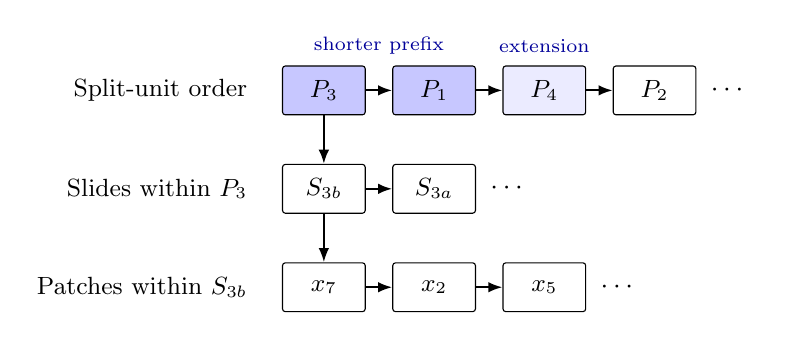
\begin{tikzpicture}[
    unit/.style={draw, rounded corners=1pt, minimum width=1.05cm, minimum height=0.62cm, font=\small},
    hierarchy/.style={font=\small, anchor=east},
    arrow/.style={-{Latex[length=1.8mm]}, thick}
  ]
    \node[hierarchy] at (-0.55,1.25) {Split-unit order};
    \node[unit, fill=blue!22] (p3) at (0.3,1.25) {$P_3$};
    \node[unit, fill=blue!22] (p1) at (1.7,1.25) {$P_1$};
    \node[unit, fill=blue!8] (p4) at (3.1,1.25) {$P_4$};
    \node[unit] (p2) at (4.5,1.25) {$P_2$};
    \node at (5.45,1.25) {$\cdots$};
    \draw[arrow] (p3) -- (p1);
    \draw[arrow] (p1) -- (p4);
    \draw[arrow] (p4) -- (p2);
    \node[font=\scriptsize, blue!60!black] at (1.0,1.82) {shorter prefix};
    \node[font=\scriptsize, blue!60!black] at (3.1,1.82) {extension};

    \node[hierarchy] at (-0.55,0) {Slides within $P_3$};
    \node[unit] (s3b) at (0.3,0) {$S_{3b}$};
    \node[unit] (s3a) at (1.7,0) {$S_{3a}$};
    \node at (2.65,0) {$\cdots$};
    \draw[arrow] (s3b) -- (s3a);
    \draw[arrow] (p3.south) -- (s3b.north);

    \node[hierarchy] at (-0.55,-1.25) {Patches within $S_{3b}$};
    \node[unit] (x7) at (0.3,-1.25) {$x_7$};
    \node[unit] (x2) at (1.7,-1.25) {$x_2$};
    \node[unit] (x5) at (3.1,-1.25) {$x_5$};
    \node at (4.05,-1.25) {$\cdots$};
    \draw[arrow] (x7) -- (x2);
    \draw[arrow] (x2) -- (x5);
    \draw[arrow] (s3b.south) -- (x7.north);
  \end{tikzpicture}
  \caption{Hierarchy behind one construction ordering. A seed fixes the split-unit sequence and the local slide and patch sequences. The darker unit boxes form a shorter prefix; the lighter third box is added, without replacing earlier units, when the prefix is extended.}
  \label{fig:construction-hierarchy}
\end{figure}

\noindent Because every larger pilot level extends the preceding prefix, adjacent levels are paired within an ordering and evaluated on the same natural-validation cohort. The smallest level whose next increment changes mean balanced accuracy by less than \num{0.01} and every class recall by less than \num{0.02} in all three orderings is the \emph{stability floor}; if none qualifies, the largest candidate is used.\footnote{No pilot level is exempt from the caps. A level is dropped from the curve when no quota satisfies both caps for every construction seed---e.g., the \num{5}\% slide cap needs at least 20 contributing slides, so a class whose split units mostly contribute a single slide can leave levels below 20 infeasible. Dropped levels are recorded in the frozen pilot report.}

The definitive minimum is the larger of this empirical stability floor and a prespecified design floor. Each class must contain at least 10 split units and 20 slides, or 20 slides when split unit and slide coincide, and any class-aware batch or set must contain at least two distinct same-class units. The 10-unit and 20-slide values are not estimated performance thresholds: they are the smallest counts compatible with the 10\% split-unit and 5\% slide contribution caps, respectively. The same 20-slide lower bound is retained for MIL to keep slide-based method comparisons outside a five-example regime even though MIL has no separate 5\% slide cap. A requested severity is reduced to the largest allocation satisfying both floors; a dataset--regime is excluded if even its balanced condition fails them. Pilot quotas, curves, seeds, and resulting floors are frozen and reported with the definitive manifests.

\subsection{Severity profiles and tail assignments}
A binary task needs only a head and a tail count, but a multiclass task also needs a rule for the classes between those extremes. The exponential construction places the $K$ class supports at equal intervals on a logarithmic scale. For a locked order from head ($i=0$) to tail ($i=K-1$), it assigns weights
\begin{equation}
  w_i(\rho_{\mathrm{target}})=\rho_{\mathrm{target}}^{-i/(K-1)},\qquad
  n_i^*=T\frac{w_i(\rho_{\mathrm{target}})}{\sum_{j=0}^{K-1}w_j(\rho_{\mathrm{target}})},
  \quad i=0,\ldots,K-1.
  \label{eq:construction}
\end{equation}
\noindent so the head-to-tail ratio is exactly $\rho_{\mathrm{target}}$ before integer rounding. For example, with four classes and $\rho_{\mathrm{target}}=100$, the unnormalized weights are approximately $1,0.215,0.046,$ and $0.01$; the two body classes lie geometrically between the head and tail instead of being assigned ad hoc counts. Binary targets use $n_{\mathrm{head}}^*/n_{\mathrm{tail}}^*=\rho_{\mathrm{target}}$ directly. The same exponential rule is applied to every multiclass dataset--regime, so a given $\rho_{\mathrm{target}}$ denotes the same allocation shape in each of them.

The values $n_i^*$ are real-valued targets, whereas a manifest must contain whole patches or slides. \emph{Constrained integer allocation} converts them into usable class counts. Each target is rounded to the nearest integer and clipped to the class's support floor and available unique support. If the rounded counts do not sum to $T$, units are added to or removed from the classes with the largest rounding residuals until the total is exact. The resulting integers $n_i$ therefore satisfy $\sum_i n_i=T$ and every class-specific lower and upper bound while remaining close to the exponential targets under this deterministic adjustment.

Counts determine how many units a class contributes; construction orderings determine which units they are. One master ordering is created per class at each hierarchy level. Every condition selects a deterministic prefix, or a split-unit-round-robin extension of a prefix, from these same orderings. For patch classification, all fixed-pool split units and slides contribute before additional patches are allocated; for MIL, slides are selected by cycling through the split-unit prefix before revisiting a unit.

If a target ratio is infeasible, the same rule is applied to every dataset and regime: use the largest attainable ratio and report the requested ratio, achieved ratio, limiting class, realized counts, and binding support floor. Validation or test support is never reduced to manufacture feasibility. This general fallback is especially relevant to high-$K$ tasks, where an exponential profile must allocate support to many intermediate classes as well as the tail; it is not a dataset-specific exception. A stable lower-severity condition is preferred to a nominal $\rho=100$ condition supported by only a few independent units.

The fallback has a limit: a moderate or severe condition whose realized allocation is indistinguishable from the balanced condition---achieved ratio within a small tolerance of 1, or realized counts identical to the balanced manifest---is not a lower-severity instance of the intended contrast but a null one, since the imbalance intervention did not occur. Such a condition is reported as degenerate rather than fitted and averaged with genuine moderate or severe conditions from other splits or assignments, and it is excluded from the imbalance deficit and recovery estimands in Section~\ref{sec:recovery}. Its requested ratio, achieved ratio, limiting class, and binding support floor are recorded alongside the exclusion, using the same fields every condition already reports.

The profile determines support by rank, so a second decision maps semantic classes to those ranks. Using only one mapping would confound a class's intrinsic difficulty with its position in the tail. Multiclass targets therefore use three locked assignments where feasible: (i) classes ordered by clinical meaning or native support, (ii) the reverse of that order for ordinal targets or a one-position rotation for nominal targets, and (iii) one distinct random permutation drawn and recorded before fitting. Figure~\ref{fig:tail-assignments} illustrates the nominal case. Binary tasks use both head--tail orientations. If support constraints make an assignment infeasible at the shared $T$, the achieved allocation is reported and the assignment is omitted only under a prespecified feasibility rule.

\begin{figure}[ht]
  \centering
  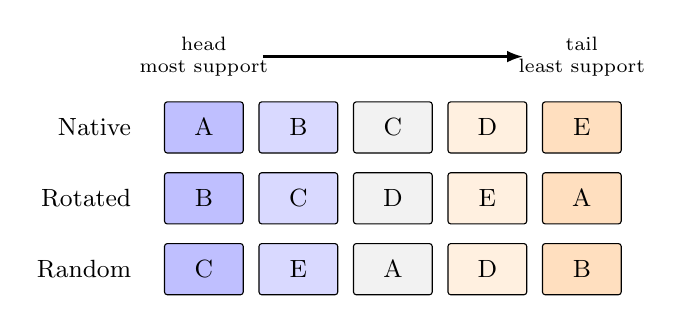
\begin{tikzpicture}[
    cls/.style={draw, rounded corners=1pt, minimum width=1.0cm, minimum height=0.65cm, font=\small},
    row/.style={font=\small, anchor=east},
    rank/.style={font=\scriptsize, align=center}
  ]
    \node[rank] at (0,1.55) {head\\most support};
    \node[rank] at (4.8,1.55) {tail\\least support};
    \draw[-{Latex[length=2mm]}, thick] (0.75,1.55) -- (4.05,1.55);

    \node[row] at (-0.8,0.65) {Native};
    \node[row] at (-0.8,-0.25) {Rotated};
    \node[row] at (-0.8,-1.15) {Random};

    \node[cls, fill=blue!25] at (0,0.65) {A};
    \node[cls, fill=blue!15] at (1.2,0.65) {B};
    \node[cls, fill=gray!10] at (2.4,0.65) {C};
    \node[cls, fill=orange!12] at (3.6,0.65) {D};
    \node[cls, fill=orange!25] at (4.8,0.65) {E};

    \node[cls, fill=blue!25] at (0,-0.25) {B};
    \node[cls, fill=blue!15] at (1.2,-0.25) {C};
    \node[cls, fill=gray!10] at (2.4,-0.25) {D};
    \node[cls, fill=orange!12] at (3.6,-0.25) {E};
    \node[cls, fill=orange!25] at (4.8,-0.25) {A};

    \node[cls, fill=blue!25] at (0,-1.15) {C};
    \node[cls, fill=blue!15] at (1.2,-1.15) {E};
    \node[cls, fill=gray!10] at (2.4,-1.15) {A};
    \node[cls, fill=orange!12] at (3.6,-1.15) {D};
    \node[cls, fill=orange!25] at (4.8,-1.15) {B};
  \end{tikzpicture}
  \caption{Illustrative tail assignments for a five-class nominal target. Columns are support ranks fixed by the severity profile; rows change which semantic class occupies each rank. Ordinal targets reverse rather than rotate the second assignment.}
  \label{fig:tail-assignments}
\end{figure}

The random quantities are separated into five seed families so that changing one source of variation does not silently change another. Table~\ref{tab:seed-families} defines their roles.

\begin{table}[H]
  \centering
  \footnotesize
  \begin{tabularx}{\linewidth}{@{}l>{\raggedright\arraybackslash}p{0.37\linewidth}>{\raggedright\arraybackslash}X@{}}
    \toprule
    Seed family & Determines & Prespecified use \\
    \midrule
    Split-unit partition & Membership of the training, validation, and test cohorts & Three locked patient- or case-disjoint splits \\
    Tail assignment & Mapping of semantic classes to head--tail support ranks & Recorded clinical/native, reversed/rotated, and random mappings \\
    Construction & Split-unit, slide, and patch orderings and the selected evidence & Three pilot orderings and a disjoint fourth ordering for definitive manifests \\
    Initialization & Parameter initialization and optimization randomness & Two tuning seeds and five disjoint confirmation seeds \\
    Resampling & Bootstrap draws and permutation swaps & Uncertainty intervals and hypothesis tests only \\
    \bottomrule
  \end{tabularx}
  \caption{Seed families and their non-overlapping roles in the benchmark.}
  \label{tab:seed-families}
\end{table}

\noindent No seed is chosen based on test performance. The size-matched balanced manifest and its trained CE baseline are shared by all tail assignments within a split.\footnote{At $\rho_{\mathrm{target}}=1$, every class receives equal support. Permuting semantic classes across support ranks therefore leaves the allocation unchanged, so tail assignment is not a meaningful factor for the balanced condition.} The same balanced predictions enter every assignment-specific deficit and are represented once in resampling data, avoiding duplicated balanced fits, bootstrap records, and artificial assignment variability.

\subsection{Mitigation methods}
\label{sec:methods}
Table~\ref{tab:roster} lists only the methods evaluated in this benchmark. CE and MIL CE are the size-matched no-mitigation references. Method objectives, tested adaptations, ablations, defaults, and fidelity qualifications are defined exclusively in the companion methods report \citep{queisler2026imbalanceMethods}.

\begin{table}[ht]
  \centering
  \footnotesize
  \begin{tabularx}{\linewidth}{@{}>{\raggedright\arraybackslash}p{0.23\linewidth}>{\raggedright\arraybackslash}p{0.43\linewidth}>{\raggedright\arraybackslash}X@{}}
    \toprule
    Family & Tested methods & Regime \\
    \midrule
    No-mitigation reference & CE; MIL CE & Patch; WSI \\
    Data-level sampling and augmentation & Balanced sampling; RankMix-inspired feature mixing & Both for sampling; WSI for RankMix-inspired \\
    Losses and prior correction & Weighted CE; focal loss; train-time and post-hoc logit adjustment; CFAL & Both, except CFAL patch only \\
    Hybrid sampling--loss & CE + soft F1; CE + soft MCC; OKO set learning; MDE-inspired dual-expert MIL & Patch for CE hybrids and OKO; WSI for MDE-inspired \\
    Representation and architecture & cRT; SC-MIL & Both for cRT; WSI for SC-MIL \\
    \bottomrule
  \end{tabularx}
  \caption{Prespecified method roster, using the same intervention-level taxonomy as the companion methods report. ``Both'' means the patch and WSI implementations defined there, not a comparison of their raw scores.}
  \label{tab:roster}
\end{table}

\subsection{Training, selection, and replication}
\label{sec:training}
The frozen encoder, classifier family, optimizer family, batch definition, augmentation, and numerical precision are held fixed within a regime. Training is budgeted only in optimizer updates; epochs are neither a stopping rule nor a unit of comparison. Let $B$ be the regime's locked batch size and $T$ the common controlled support. A single-stage model receives
\begin{equation}
  U=30\left\lceil\frac{T}{B}\right\rceil
  \label{eq:update-budget}
\end{equation}
updates, corresponding to 30 reference passes through $T$ examples under ordinary sampling. Balanced sampling, replacement, synthetic bags, and dual loaders do not change $U$. RankMix receives $U$ teacher updates and, after reinitialization, $U$ student updates. cRT receives $U$ stage-one updates and $\lceil0.2U\rceil$ stage-two classifier updates. MDE performs $U$ joint updates, each consuming its prespecified natural and balanced minibatches. The natural anchor uses the same formula with its own support and is descriptive. Processed examples, unique-example exposures, and updates are all reported. Each run stores validation metrics at fixed update intervals. The selected checkpoint maximizes natural-validation balanced accuracy, with macro F1 and then lower NLL as deterministic tie-breakers. Test predictions are produced once from that locked checkpoint.

Hyperparameter comparisons are bounded by a common validation-search budget rather than by restricting every method to one tuned quantity. For each trainable mitigation method, its four-value imbalance-specific grid is crossed with the common four-value learning-rate grid in Appendix~\ref{app:controls}, yielding at most 16 candidate configurations. This joint search accommodates interactions between a method's objective and optimization dynamics while holding the optimizer family, weight decay, architecture, batch definition, and all other training parameters fixed. CE and methods without a meaningful imbalance-specific control evaluate the four learning rates without introducing an artificial search dimension. Train-time logit adjustment is tuned jointly over $\tau$ and learning rate; post-hoc logit adjustment inherits the selected CE model and tunes only $\tau$ because it performs no gradient optimization.

Every hyperparameter candidate is fitted with the same two tuning initialization seeds for each prespecified split-unit partition and tail assignment. Selection is performed separately for each method, dataset, prediction regime, and imbalance severity. Within each such selection unit, natural-validation balanced accuracy is averaged across both tuning seeds, all tuning splits, and all tail assignments. The configuration with the highest aggregate value is selected; macro F1 and then lower NLL are deterministic tie-breakers. The chosen configuration is locked before any of the five disjoint confirmation initialization seeds are fitted and before test evaluation. Tuning runs never enter confirmation effect estimates. For cRT, stage one inherits the selected CE configuration, while the stage-two classifier learning rate is selected separately from the common grid. Temperature scaling, when reported, fits one positive scalar on natural-validation NLL after model and checkpoint selection and applies it unchanged to test logits \citep{guo2017calibration}.

A \emph{controlled contrast} is the difference between two matched runs, such as balanced CE versus imbalanced CE or a mitigation method versus imbalanced CE. The two runs use the same split-unit partition, tail assignment, confirmation-seed index, and held-out cases, so the contrast does not mix the intended change with a different cohort or replication. Each locked partition and tail assignment is repeated with the five confirmation seeds. Exactly three split-unit partition seeds are used; a dataset--regime unable to produce all three valid splits under the independent-support floors is excluded from the corresponding confirmatory analysis. The split counts, support floors, condition manifests, tuning and confirmation seeds, method grids, and update budgets are frozen in the signed analysis manifest before the first definitive fit. The unit of replication and all missing or failed runs are reported. A failed run is not silently replaced using a test-informed seed.

Computational cost is separated into validation search and locked-configuration fitting. Resource use is summarized by wall-clock training time, accelerator-hours, and peak accelerator memory. Model size is reported as total and trainable parameter counts, while data exposure is reported as effective passes through unique training examples. Costs include every method-specific stage, including both cRT stages, but exclude the one-time frozen-feature extraction shared by all methods. Hardware and software environments are recorded with each run.

\subsection{Scope and limitations}
The design isolates training-distribution effects under frozen Virchow2 representations; it does not establish how end-to-end encoder fine-tuning would respond to imbalance. Constructed tails improve causal interpretability but need not reproduce referral pathways or biological prevalence. A shared $T$ controls data volume at the cost of discarding some available training examples, which is why the full natural condition is retained as a descriptive anchor. Some methods change more than one mechanism, so the study supports method-level comparisons rather than universal causal claims about sampling or loss design. The locked update budget equalizes optimizer steps but not information exposure: RankMix consumes teacher and student passes, MDE draws a natural and a balanced minibatch per update, and post-hoc logit adjustment performs no gradient optimization at all, so method comparisons are made at equal update budget with exposure and cost reported alongside, not at equal data throughput. MIL instance counts likewise vary with the eligible tissue area of each selected slide; processed instances, memory, and runtime are therefore reported rather than equalized by truncating bags. The number of independent split units, not the number of patches, limits inference. All imbalance-robustness findings are additionally conditional on the geometry of a single frozen encoder; whether the same deficits and recoveries hold under a different foundation representation is outside the present scope. Finally, calibration on a natural held-out cohort is conditional on that cohort's prevalence and should not be transported to a new deployment population without explicit prior-shift analysis.

\section{Evaluation and Statistical Analysis}
\label{sec:analysis}
Evaluation proceeds from description to explanation. It first measures which classes are predicted correctly, then reports PANDA-specific ordinal error and examines probability quality. It next determines whether imbalance caused a deficit, quantifies split-unit-clustered uncertainty, and tests recovery while accounting for multiple comparisons. Finally, RQ3 explores why damage and recovery differ across controlled comparisons. All endpoints, decision rules, and inferential families are fixed before test evaluation.

\subsection{Discrimination endpoints and aggregation units}
The primary endpoint is balanced accuracy, equal to macro recall for single-label multiclass prediction. Secondary discrimination outcomes are macro F1; per-class recall and F1; and head, body, and tail recall under the locked assignment. Classes are ranked by allocated training support: the first $\lceil K/3\rceil$ ranks are head, the last $\lceil K/3\rceil$ are tail, and intervening ranks are body; binary tasks have one head and one tail and no body. Ties follow the locked class ordering. Overall accuracy is descriptive. Patch predictions are summarized in two ways: patch-micro estimates treat eligible patches as predictions while uncertainty remains split-unit-clustered, and slide/case-macro estimates first aggregate the metric contribution within each slide or split unit so that heavily tiled slides do not dominate. WSI outcomes are slide-level with patient clustering where patients contribute multiple slides and WSI/case clustering otherwise.

\subsection{Ordinal outcomes for PANDA}
Balanced accuracy treats every wrong class as an error of the same kind. PANDA WSI prediction is the only ordinal task in the benchmark, so it also receives two dataset-specific secondary outcomes that use the distance between ISUP grades. These measures complement rather than replace the common discrimination endpoints.

Let $N$ be the number of held-out biopsies and $C$ the number of grades. Let $O_{ab}$ be the observed confusion-matrix count for true grade $a$ and predicted grade $b$. The count expected under independent true and predicted grades is $E_{ab}=O_{a\cdot}O_{\cdot b}/N$, which retains the observed marginal grade frequencies. With $a,b\in\{0,\ldots,C-1\}$ and quadratic disagreement weight $w_{ab}=(a-b)^2/(C-1)^2$, quadratic-weighted kappa is
\begin{equation}
  \kappa_{\mathrm{QW}}
  =1-\frac{\sum_{a=0}^{C-1}\sum_{b=0}^{C-1}w_{ab}O_{ab}}
  {\sum_{a=0}^{C-1}\sum_{b=0}^{C-1}w_{ab}E_{ab}}.
  \label{eq:qwk}
\end{equation}
\noindent A value of 1 denotes perfect grade agreement, 0 is the agreement expected from the marginal grade frequencies, and negative values indicate more weighted disagreement than expected by chance. Ordinal mean absolute error (MAE) is
\begin{equation}
  \mathrm{MAE}_{\mathrm{ord}}
  =\frac{1}{N}\sum_{i=1}^{N}|g_i-\widehat g_i|,
  \label{eq:ordinal-mae}
\end{equation}
\noindent where $g_i$ and $\widehat g_i$ are the true and predicted ISUP grades. It reports the average distance in grade levels and is lower-is-better. Kappa emphasizes agreement beyond the observed marginals, whereas MAE has the direct interpretation of grades missed per biopsy.

\subsection{Probability quality and calibration}
Discrimination metrics depend mainly on which class receives the highest score. Probability-quality metrics instead evaluate the full predicted distribution and whether confidence is compatible with observed outcomes. Tail-group macro negative log likelihood (NLL) is the co-primary calibration endpoint used by the recovery gate in Section~\ref{sec:recovery}. Natural-prevalence NLL, macro NLL, the Brier score, expected calibration error (ECE), and reliability diagrams provide complementary secondary views.

Let $N$ denote the number of held-out predictions in an aggregation unit, $C$ the number of classes, $y_i\in\{1,\ldots,C\}$ the true label, and $\hat{\mathbf{p}}_i\in[0,1]^C$ the predicted probability vector. Write $Y_i$ for the one-hot encoding of $y_i$.

Table~\ref{tab:score-variants} fixes which score variant enters each endpoint. For ordinary CE,
post-hoc logit adjustment, and train-time logit adjustment, the target-prior variant is the
correction defined in the companion methods report, using the natural-validation prior for the
corresponding test split. For every other method, the target-prior variant equals its raw logits.

\begin{table}[ht]
  \centering
  \small
  \begin{tabularx}{\linewidth}{@{}p{0.36\linewidth}X@{}}
    \toprule
    Endpoint or output & Score variant \\
    \midrule
    Balanced accuracy and all other discrimination endpoints
      & Balanced-decision logits: $z^{\mathrm{CE}}-\tau\log\widehat\pi$ for post-hoc logit adjustment; raw model logits for train-time logit adjustment and every other method. \\
    Tail-NLL deficit gate and tail-NLL recovery
      & Target-prior-corrected probabilities before temperature scaling. \\
    Reported NLL, Brier score, ECE, and reliability diagrams
      & Target-prior-corrected probabilities before temperature scaling; raw probabilities are retained as a separately labelled diagnostic. \\
    Temperature-scaled calibration outputs
      & Target-prior-corrected logits divided by one positive temperature fitted on natural-validation NLL and applied unchanged to test; these secondary outputs do not enter either recovery gate. \\
    \bottomrule
  \end{tabularx}
  \caption{Canonical mapping from evaluation endpoints to score variants.}
  \label{tab:score-variants}
\end{table}

\paragraph{Negative log likelihood.}
Natural-prevalence negative log likelihood (NLL), also called multiclass log loss, is
\begin{equation}
  \mathrm{NLL}=-\frac{1}{N}\sum_{i=1}^{N}\log \hat{p}_{i,y_i}.
  \label{eq:nll}
\end{equation}
\noindent Lower NLL indicates that more probability mass is assigned to the true class. The implementation clips $\hat{p}_{i,y_i}$ to $[10^{-12},1]$ before taking the logarithm. To prevent common classes from dominating probability-quality summaries, class-conditional NLL and macro NLL are
\begin{equation}
  \mathrm{NLL}_c=-\frac{1}{N_c}\sum_{i:y_i=c}\log \hat{p}_{ic},
  \qquad
  \mathrm{NLL}_{\mathrm{macro}}=\frac{1}{C}\sum_{c=1}^{C}\mathrm{NLL}_c,
  \label{eq:macro-nll}
\end{equation}
\noindent where $N_c$ is the number of held-out predictions from class $c$. Natural-prevalence NLL is the deployment-facing summary for the observed held-out cohort; macro NLL and unweighted head, body, and tail averages of $\mathrm{NLL}_c$ are tail-sensitive summaries.

\paragraph{Multiclass Brier score.}
The multiclass Brier score penalizes squared error across the full predicted distribution \citep{brier1950verification}:
\begin{equation}
  \mathrm{BS}=\frac{1}{N}\sum_{i=1}^{N}
  \left\|\hat{\mathbf{p}}_i-Y_i\right\|_2^2.
  \label{eq:brier}
\end{equation}
\noindent Lower values indicate better probability quality. The natural-prevalence score averages this error over the complete held-out cohort. Classwise scores apply the same full-distribution error only to predictions with $y_i=c$. Their unweighted averages provide head, body, and tail summaries.

\paragraph{Expected calibration error.}
For each prediction, let $\hat{y}_i=\arg\max_c\hat{p}_{ic}$ and $q_i=\max_c\hat{p}_{ic}$. Expected calibration error (ECE) partitions confidence into $B=10$ fixed equal-width bins on $[0,1]$ and compares mean confidence with empirical accuracy in each nonempty bin \citep{naeini2015obtaining}:
\begin{equation}
  \mathrm{ECE}=\sum_{b=1}^{B}\frac{|I_b|}{N}
  \left|\frac{1}{|I_b|}\sum_{i\in I_b}\mathbb{1}[\hat{y}_i=y_i]
  -\frac{1}{|I_b|}\sum_{i\in I_b}q_i\right|,
  \label{eq:ece}
\end{equation}
\noindent where $I_b$ contains the predictions assigned to bin $b$. ECE is secondary because it depends on binning and can be unstable with small classwise samples; its bootstrap uncertainty uses the same fixed bins and split-unit weights as the other endpoints. Reliability diagrams show the binwise confidence--accuracy relation overall and for the tail group.

Because checkpoints and hyperparameters are selected for natural-validation balanced accuracy, all probability-quality results describe discrimination-selected models rather than models optimized for calibration. The output semantics and prior-correction formulas of individual methods are defined in the companion methods report \citep{queisler2026imbalanceMethods}.

\subsection{From imbalance deficit to mitigation recovery}
\label{sec:recovery}
Recovery is meaningful only when imbalance has first caused a measurable loss. The analysis therefore proceeds in two stages: compare size-matched balanced and imbalanced CE, then evaluate mitigation only on an endpoint that shows sufficiently large and statistically supported harm. One \emph{comparison unit} is a fixed dataset, prediction regime, imbalance severity, and tail assignment. A \emph{gate} is the prespecified eligibility rule that routes such a unit to the relevant recovery analysis; it is not a learned model component.

For a higher-is-better metric $M$, define the imbalance-induced deficit and recovery fraction at each imbalanced condition as
\begin{equation}
  \begin{aligned}
    D_M &= M(\text{balanced CE})-M(\text{imbalanced CE}),\\
    R_M &= \frac{M(\text{method on imbalanced data})
      -M(\text{imbalanced CE})}{D_M}.
  \end{aligned}
  \label{eq:recovery}
\end{equation}
$R_M=0$ denotes no recovery, $R_M=1$ recovery to the size-matched balanced CE reference, $R_M<0$ further deterioration, and $R_M>1$ performance beyond that reference. Because the balanced reference draws more unique tail independent units than any imbalanced condition at the same $T$, methods that only reweight or recalibrate the imbalanced manifest cannot restore tail evidence that was never sampled; for that family $R_M<1$ may reflect an information ceiling rather than method failure, whereas resampling and synthesis methods are the only family for which $R_M=1$ is mechanically attainable. The full natural condition is descriptive and never enters $D_M$ or $R_M$.

\begin{figure}[H]
  \centering
  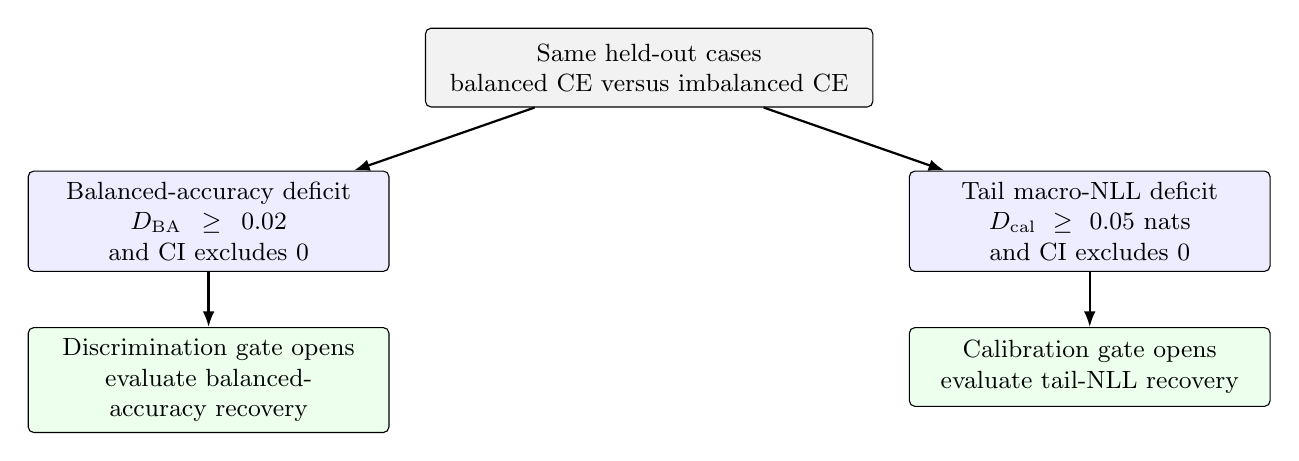
\begin{tikzpicture}[
    box/.style={draw, rounded corners=2pt, align=center, inner sep=4pt, font=\small, text width=4.3cm, minimum height=1.0cm},
    start/.style={box, fill=gray!10, text width=5.4cm},
    route/.style={box, fill=blue!7},
    result/.style={box, fill=green!7},
    arrow/.style={-{Latex[length=2mm]}, thick}
  ]
    \node[start] (contrast) {Same held-out cases\\balanced CE versus imbalanced CE};
    \node[route, below left=0.8cm and 0.45cm of contrast] (ba) {Balanced-accuracy deficit\\$D_{\mathrm{BA}}\geq0.02$ and CI excludes 0};
    \node[route, below right=0.8cm and 0.45cm of contrast] (cal) {Tail macro-NLL deficit\\$D_{\mathrm{cal}}\geq0.05$ nats and CI excludes 0};
    \node[result, below=0.7cm of ba] (barec) {Discrimination gate opens\\evaluate balanced-accuracy recovery};
    \node[result, below=0.7cm of cal] (calrec) {Calibration gate opens\\evaluate tail-NLL recovery};
    \draw[arrow] (contrast) -- (ba);
    \draw[arrow] (contrast) -- (cal);
    \draw[arrow] (ba) -- (barec);
    \draw[arrow] (cal) -- (calrec);
  \end{tikzpicture}
  \caption{Routing from an imbalance deficit to mitigation analysis. A comparison unit can enter through either gate or both. If neither rule is met, its CE deficits are still reported, but a recovery ratio is not interpreted. CI denotes the paired 95\% confidence interval.}
  \label{fig:gate-routing}
\end{figure}

The \emph{discrimination gate} opens when the CE balanced-accuracy deficit is at least \num{0.02} and its paired 95\% confidence interval excludes zero. The \emph{calibration gate} opens when the CE tail-group macro-NLL deficit, $\mathrm{NLL}_{\mathrm{tail}}(\mathrm{imbalanced\ CE})-\mathrm{NLL}_{\mathrm{tail}}(\mathrm{balanced\ CE})$, is at least \num{0.05} nats with a paired 95\% confidence interval excluding zero. Both rules are computed from CE runs on the same held-out cases before any mitigation method is compared. A comparison unit entering through the discrimination gate is evaluated for balanced-accuracy recovery; one entering through the calibration gate is evaluated for tail-calibration recovery; it may enter through both.

The two routes preserve an important distinction. Strong frozen features may leave balanced accuracy nearly intact while imbalance still biases tail probabilities, in which case a single discrimination rule would exclude methods designed to correct class priors. Conversely, the gates avoid unstable recovery ratios when no meaningful damage exists to recover. All CE deficits on both axes remain reported, including units that fail both rules. For the lower-is-better calibration axis, the sign-corrected deficit $D_{\mathrm{cal}}=\mathrm{NLL}_{\mathrm{tail}}(\mathrm{imbalanced\ CE})-\mathrm{NLL}_{\mathrm{tail}}(\mathrm{balanced\ CE})$ is the denominator and the method's tail-NLL improvement over imbalanced CE is the numerator, so Equation~\eqref{eq:recovery} retains the same interpretation. Recovery for other secondary metrics is descriptive and does not reopen a comparison unit that fails both gates.

\subsection{Uncertainty from split-unit resampling}
A \emph{bootstrap} approximates sampling uncertainty by repeatedly constructing hypothetical test cohorts from the observed split units: patients or participants where available, and the biopsy/WSI for PANDA and CAMELYON16. Sampling is performed \emph{with replacement}, so one split unit can be selected more than once or not selected at all. The metric is recomputed for every replicate, and the spread of those values shows how much the result could change under a similar case sample. Split units---not patches---are resampled because patches from one case are correlated.

\paragraph{Label-only preflight.}
Before model training, \num{10000} bootstrap replicates are constructed using only split-unit identifiers, split membership, and class labels. \emph{Label-only} means that no predictions, performance values, or method identities are used; these replicates test whether the planned resampling scheme is valid before results can influence it. The count of \num{10000} is a prespecified Monte Carlo budget. It places about 250 replicates in each 2.5\% tail of a percentile interval, reducing simulation noise in the interval endpoints while remaining inexpensive at this label-only stage.

A \emph{stratum} is a group of split units with the same observed contribution pattern. Here, that pattern records how many examples a unit contributes to each class in each test-split appearance. Units are resampled only against others in the same stratum. This preserves the observed split--class structure, including patch targets for which one case can contribute several classes. A selected unit's multiplicity is applied to all of its slides and patches in every split. Figure~\ref{fig:bootstrap-workflow} summarizes the workflow.

\begin{figure}[ht]
  \centering
  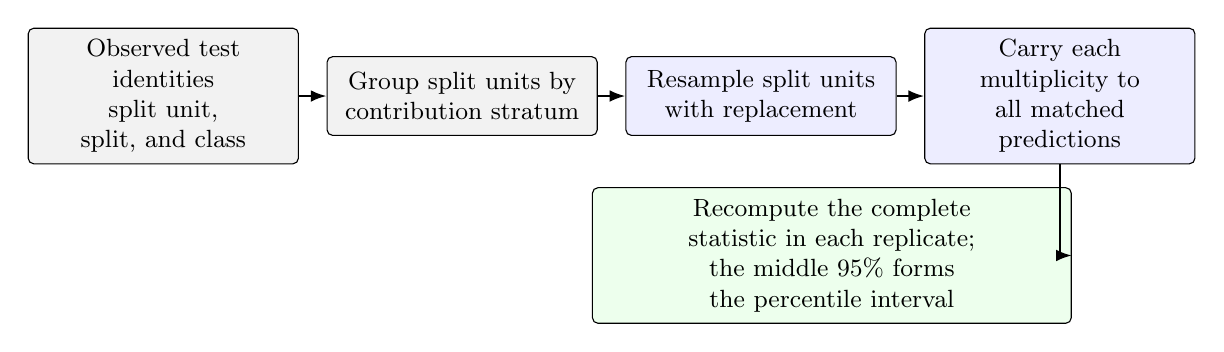
\begin{tikzpicture}[
    box/.style={draw, rounded corners=2pt, align=center, inner sep=4pt, font=\small, text width=3.15cm, minimum height=1.0cm},
    fixed/.style={box, fill=gray!10},
    sampled/.style={box, fill=blue!7},
    result/.style={box, fill=green!7, text width=5.8cm},
    arrow/.style={-{Latex[length=2mm]}, thick}
  ]
    \node[fixed] (identity) {Observed test identities\\split unit, split, and class};
    \node[fixed, right=0.35cm of identity] (strata) {Group split units by\\contribution stratum};
    \node[sampled, right=0.35cm of strata] (resample) {Resample split units\\with replacement};
    \node[sampled, right=0.35cm of resample] (weights) {Carry each multiplicity to\\all matched predictions};
    \node[result, below=0.65cm of resample, xshift=0.9cm] (interval) {Recompute the complete statistic in each replicate;\\the middle 95\% forms the percentile interval};
    \draw[arrow] (identity) -- (strata);
    \draw[arrow] (strata) -- (resample);
    \draw[arrow] (resample) -- (weights);
    \draw[arrow] (weights.south) |- (interval.east);
  \end{tikzpicture}
  \caption{Split-unit-clustered bootstrap workflow. The label-only preflight executes the identity, stratification, and resampling steps before predictions exist. After model fitting, the same paired multiplicities are applied to every matched run.}
  \label{fig:bootstrap-workflow}
\end{figure}

\noindent The preflight verifies that every original split--class cell remains represented, every split-level metric is computable, and one split unit receives the same multiplicity across all appearances. Failure of any check stops the analysis rather than causing a replicate to be silently discarded.

Resampling with replacement can still produce a replicate dominated by a few repeatedly selected cases. If split unit $i$ has class-specific bootstrap weight $v_i$, the \emph{Kish effective split-unit count}
\begin{equation}
  n_{\mathrm{Kish}}=\frac{\left(\sum_i v_i\right)^2}{\sum_i v_i^2}.
  \label{eq:kish}
\end{equation}
\noindent translates unequal case weights into the equivalent number of equally weighted split units. It decreases as weight concentrates. The preflight also records the number of unique units and the largest unit weight by split and class. If $n_{\mathrm{Kish}}<5$ in any replicate, or one unit supplies more than 50\% of a class's weight in more than 5\% of replicates, inference for that dataset--regime is designated descriptive before training. The diagnostic report and resampling seed are frozen with the analysis manifest.

\paragraph{Intervals after model fitting.}
The three split-unit partitions are fixed design repetitions and are averaged with equal weight; they are not treated as three independent cohorts. Tail assignments remain separate unless an assignment-averaged estimand is explicitly reported. Within each case-bootstrap replicate, the five matched confirmation-seed indices are also resampled as paired blocks and averaged before the splits are combined. This captures algorithmic variation without pretending that five model initializations create five additional case cohorts.

Balanced CE, imbalanced CE, and each mitigation method receive the same split-unit multiplicities and confirmation-seed draws. The complete deficit and recovery fraction, including numerator and denominator, is recomputed in each replicate. The reported 95\% percentile interval spans the 2.5th to 97.5th percentiles of the resulting distribution. Patches are never bootstrapped independently.

\subsection{Paired testing and multiplicity control}
Confidence intervals and raw effect sizes are the main evidence. Hypothesis tests provide a supporting check for the prespecified primary methods. On the discrimination axis, the tested effect is the balanced-accuracy improvement over imbalanced CE. On the calibration axis, it is the reduction in tail-group macro NLL, oriented so that positive values indicate improvement. Recovery fractions are normalized effect summaries, not test statistics.

The raw two-sided $p$-value comes from a paired split-unit-block permutation test. This test represents the null hypothesis of no method difference by repeatedly swapping the method and imbalanced-CE labels within a split unit. The same swap is used for all of that unit's slides, patches, split appearances, and matched confirmation seeds, preserving the paired design. All possible swaps are enumerated when feasible. Otherwise, \num{100000} random swaps are used with a plus-one correction; this gives a minimum attainable Monte Carlo $p$-value of approximately $10^{-5}$ and avoids reporting a simulated value of zero.

A \emph{test family} is the set of related hypotheses interpreted together. Testing many hypotheses increases the chance that at least one small $p$-value occurs by chance. Holm adjustment controls this family-wise error by ordering the raw $p$-values from smallest to largest, applying the strongest correction to the smallest value, and then proceeding stepwise with less stringent corrections. It provides this control without assuming that the tests are independent.

The confirmatory family contains weighted CE, focal loss, train-time logit adjustment, and balanced sampling. These four primary methods directly target tail support or class priors and are shared across both prediction regimes. Within one dataset and regime, the family includes every gate-passing combination of primary method, gate, severity, and tail assignment; severities are not split into separate families. Holm adjustment is applied across the testable comparisons, while gated-out comparisons are recorded as not tested. All remaining methods and all secondary classwise, calibration, and cost analyses are exploratory. They retain the same effect estimates and confidence intervals but remain outside the confirmatory correction.

\subsection{Exploratory explanation of damage and recovery (RQ3)}
RQ1 and RQ2 estimate matched effects within a dataset and task. RQ3 takes one step back and asks why some of those controlled comparisons show more damage or recovery than others. It does not predict individual patient outcomes and it does not rank mitigation methods. For damage occurrence and magnitude, one observation is a dataset, prediction regime, imbalance severity, and tail assignment. Recovery observations additionally identify the mitigation method and the discrimination or calibration gate through which the comparison entered.

\paragraph{Outcomes to explain.}
The analysis is divided into three linked questions rather than one opaque combined model:
\begin{enumerate}
  \item \textbf{Damage occurrence:} did the comparison pass either prespecified deficit gate? Every controlled comparison contributes to this binary analysis.
  \item \textbf{Damage magnitude:} how large was the signed balanced-accuracy deficit? Every comparison contributes, including those with no damage or an apparent improvement under imbalance.
  \item \textbf{Mitigation headroom:} how much of the demonstrated deficit was recovered? Only gated comparisons contribute because recovery has no stable interpretation when there is no deficit to recover.
\end{enumerate}

\noindent These three outcomes correspond directly to the sequence introduced in RQ3: occurrence, magnitude, and conditional recovery.

\paragraph{Candidate explanations.}
Only quantities available without using test outcomes are eligible as predictors. Table~\ref{tab:rq3-predictors} separates the two primary predictors from the variables used only in sensitivity analyses.

\begin{table}[ht]
  \centering
  \footnotesize
  \begin{tabularx}{\linewidth}{@{}>{\raggedright\arraybackslash}p{0.23\linewidth}>{\raggedright\arraybackslash}p{0.49\linewidth}X@{}}
    \toprule
    Predictor & Question it represents & Model role \\
    \midrule
    Achieved imbalance ratio & How extreme was the realized head--tail allocation? & Primary, log-transformed \\
    Intrinsic separability & How distinguishable are the classes in a common balanced frozen-feature reference, before condition-specific support is considered? & Primary \\
    Condition-specific learnability & What remains learnable from the exact controlled training manifest? & One-predictor sensitivity \\
    Minimum independent support & How many distinct split units or slides support the scarcest class? & One-predictor sensitivity \\
    Effective patch support & How much patch support remains after accounting for within-case redundancy? & Patch-only sensitivity \\
    Prediction regime & Does the comparison use patch classification or WSI-level MIL? & One-predictor sensitivity \\
    \bottomrule
  \end{tabularx}
  \caption{RQ3 predictors and their prespecified roles. Sensitivity predictors are fitted one at a time rather than added to the primary model.}
  \label{tab:rq3-predictors}
\end{table}

\paragraph{Measuring separability and learnability.}
Intrinsic separability holds the evidence source constant. It uses one fixed balanced reference subset per dataset, regime, and split to ask whether Virchow2 already places the classes in distinguishable regions. Condition-specific learnability changes the reference to the exact balanced or imbalanced training manifest and asks how much class information remains accessible under that condition's realized support. The distinction is between inherent feature geometry and the evidence actually retained by one constructed condition.

Both quantities are evaluated on the unchanged natural-validation cohort. Balanced $k$-nearest-neighbour (kNN) macro recall labels each validation embedding from its closest reference embeddings and gives every class equal weight. A \emph{linear probe} is a class-balanced linear classifier fitted on the frozen reference embeddings; its macro recall is the primary separability or learnability summary. Per-class nearest-neighbour error is reported descriptively to show which classes overlap. None of these diagnostics uses test labels or CE test performance. Patch probes operate on patch embeddings. WSI probes use the mean and componentwise standard deviation of a slide's eligible instances, avoiding a learned attention summary from the model being explained.

\paragraph{Sensitivity to correlated patches.}
Raw patch count can overstate evidence when many patches come from the same case. Unique split-unit and slide counts therefore remain the primary support measures. As a secondary sensitivity analysis, within-case redundancy is summarized by the intraclass correlation (ICC) of a cross-fitted class margin. An ICC near zero means that patches from the same case are no more alike than patches from different cases; an ICC near one indicates strong redundancy.

For class $c$, let $G_c$ be the number of split-unit or slide clusters, $m_{gc}$ their sizes, and $N_c=\sum_gm_{gc}$. With between-cluster and within-cluster mean squares $\mathrm{MS}_{B,c}$ and $\mathrm{MS}_{W,c}$, the unequal-cluster-size correction and ICC are
\begin{equation}
  m_{0,c}=\frac{N_c-\sum_{g=1}^{G_c}m_{gc}^2/N_c}{G_c-1},
  \qquad
  \operatorname{ICC}_c=
  \frac{\mathrm{MS}_{B,c}-\mathrm{MS}_{W,c}}
  {\mathrm{MS}_{B,c}+(m_{0,c}-1)\mathrm{MS}_{W,c}}.
  \label{eq:icc}
\end{equation}
\noindent The estimate is clipped to $[0,1]$. The corresponding effective sample size is
\begin{equation}
  N_{\mathrm{eff},c}=\frac{N_c}{1+(\overline m_c-1)\operatorname{ICC}_c},
  \label{eq:neff}
\end{equation}
\noindent where $\overline m_c$ is the arithmetic mean cluster size. The scalar margin is the fixed intrinsic linear probe's logit for class $c$ minus its largest competing logit. It is evaluated by \emph{cross-fitting}: each observation is scored only by a probe trained without it. Equations~\eqref{eq:icc}--\eqref{eq:neff} provide a patch-only sensitivity measure, not a replacement for independent-unit counts. Slide count is used directly for WSI targets, with patient count also examined when patients contribute multiple slides.

\paragraph{Three deliberately small association models.}
One model is fitted for each of the three RQ3 outcomes. The occurrence model handles the yes/no gate result; the magnitude and recovery models handle continuous outcomes. Every primary model contains exactly two predictors: the log achieved imbalance ratio and intrinsic separability. The magnitude model also uses each deficit's bootstrap standard error so that a noisy estimated deficit is not treated as an exact observation.

Comparisons from the same dataset--target group can share a baseline level of difficulty. A \emph{random intercept} allows each group to have its own starting level while estimating common associations with imbalance and separability. This adjustment is important because the analysis pools several severities and assignments from the same group. The recovery model omits method-specific effects because the small number of gated units cannot support them.

The remaining predictors in Table~\ref{tab:rq3-predictors} are fitted one at a time in separate sensitivity models. They are not combined with one another or with the two primary predictors because only a few independent dataset--target groups are available and the candidate predictors are strongly confounded. No interactions are fitted.

Parameters are estimated by maximum a posteriori (MAP) fitting: ordinary model fit is combined with weak zero-centered Gaussian priors that discourage extreme slopes and variance estimates in this small sample. A leave-one-dataset--target-group-out check then refits the magnitude model while withholding one complete group at a time. This is only a coarse stability check, not evidence of predictive generalization. TCGA-UT supplies the only genuine paired comparison between prediction regimes; the CAMELYON16, PANDA, and BRACS targets differ by regime. Model definitions, predictor roles, and priors are frozen before recovery outcomes are inspected, and all RQ3 conclusions remain hypothesis-generating.

\clearpage
\appendix
\begin{landscape}
\section{Benchmark Overview}
\label{app:overview}

\begin{figure}[H]
  \centering
  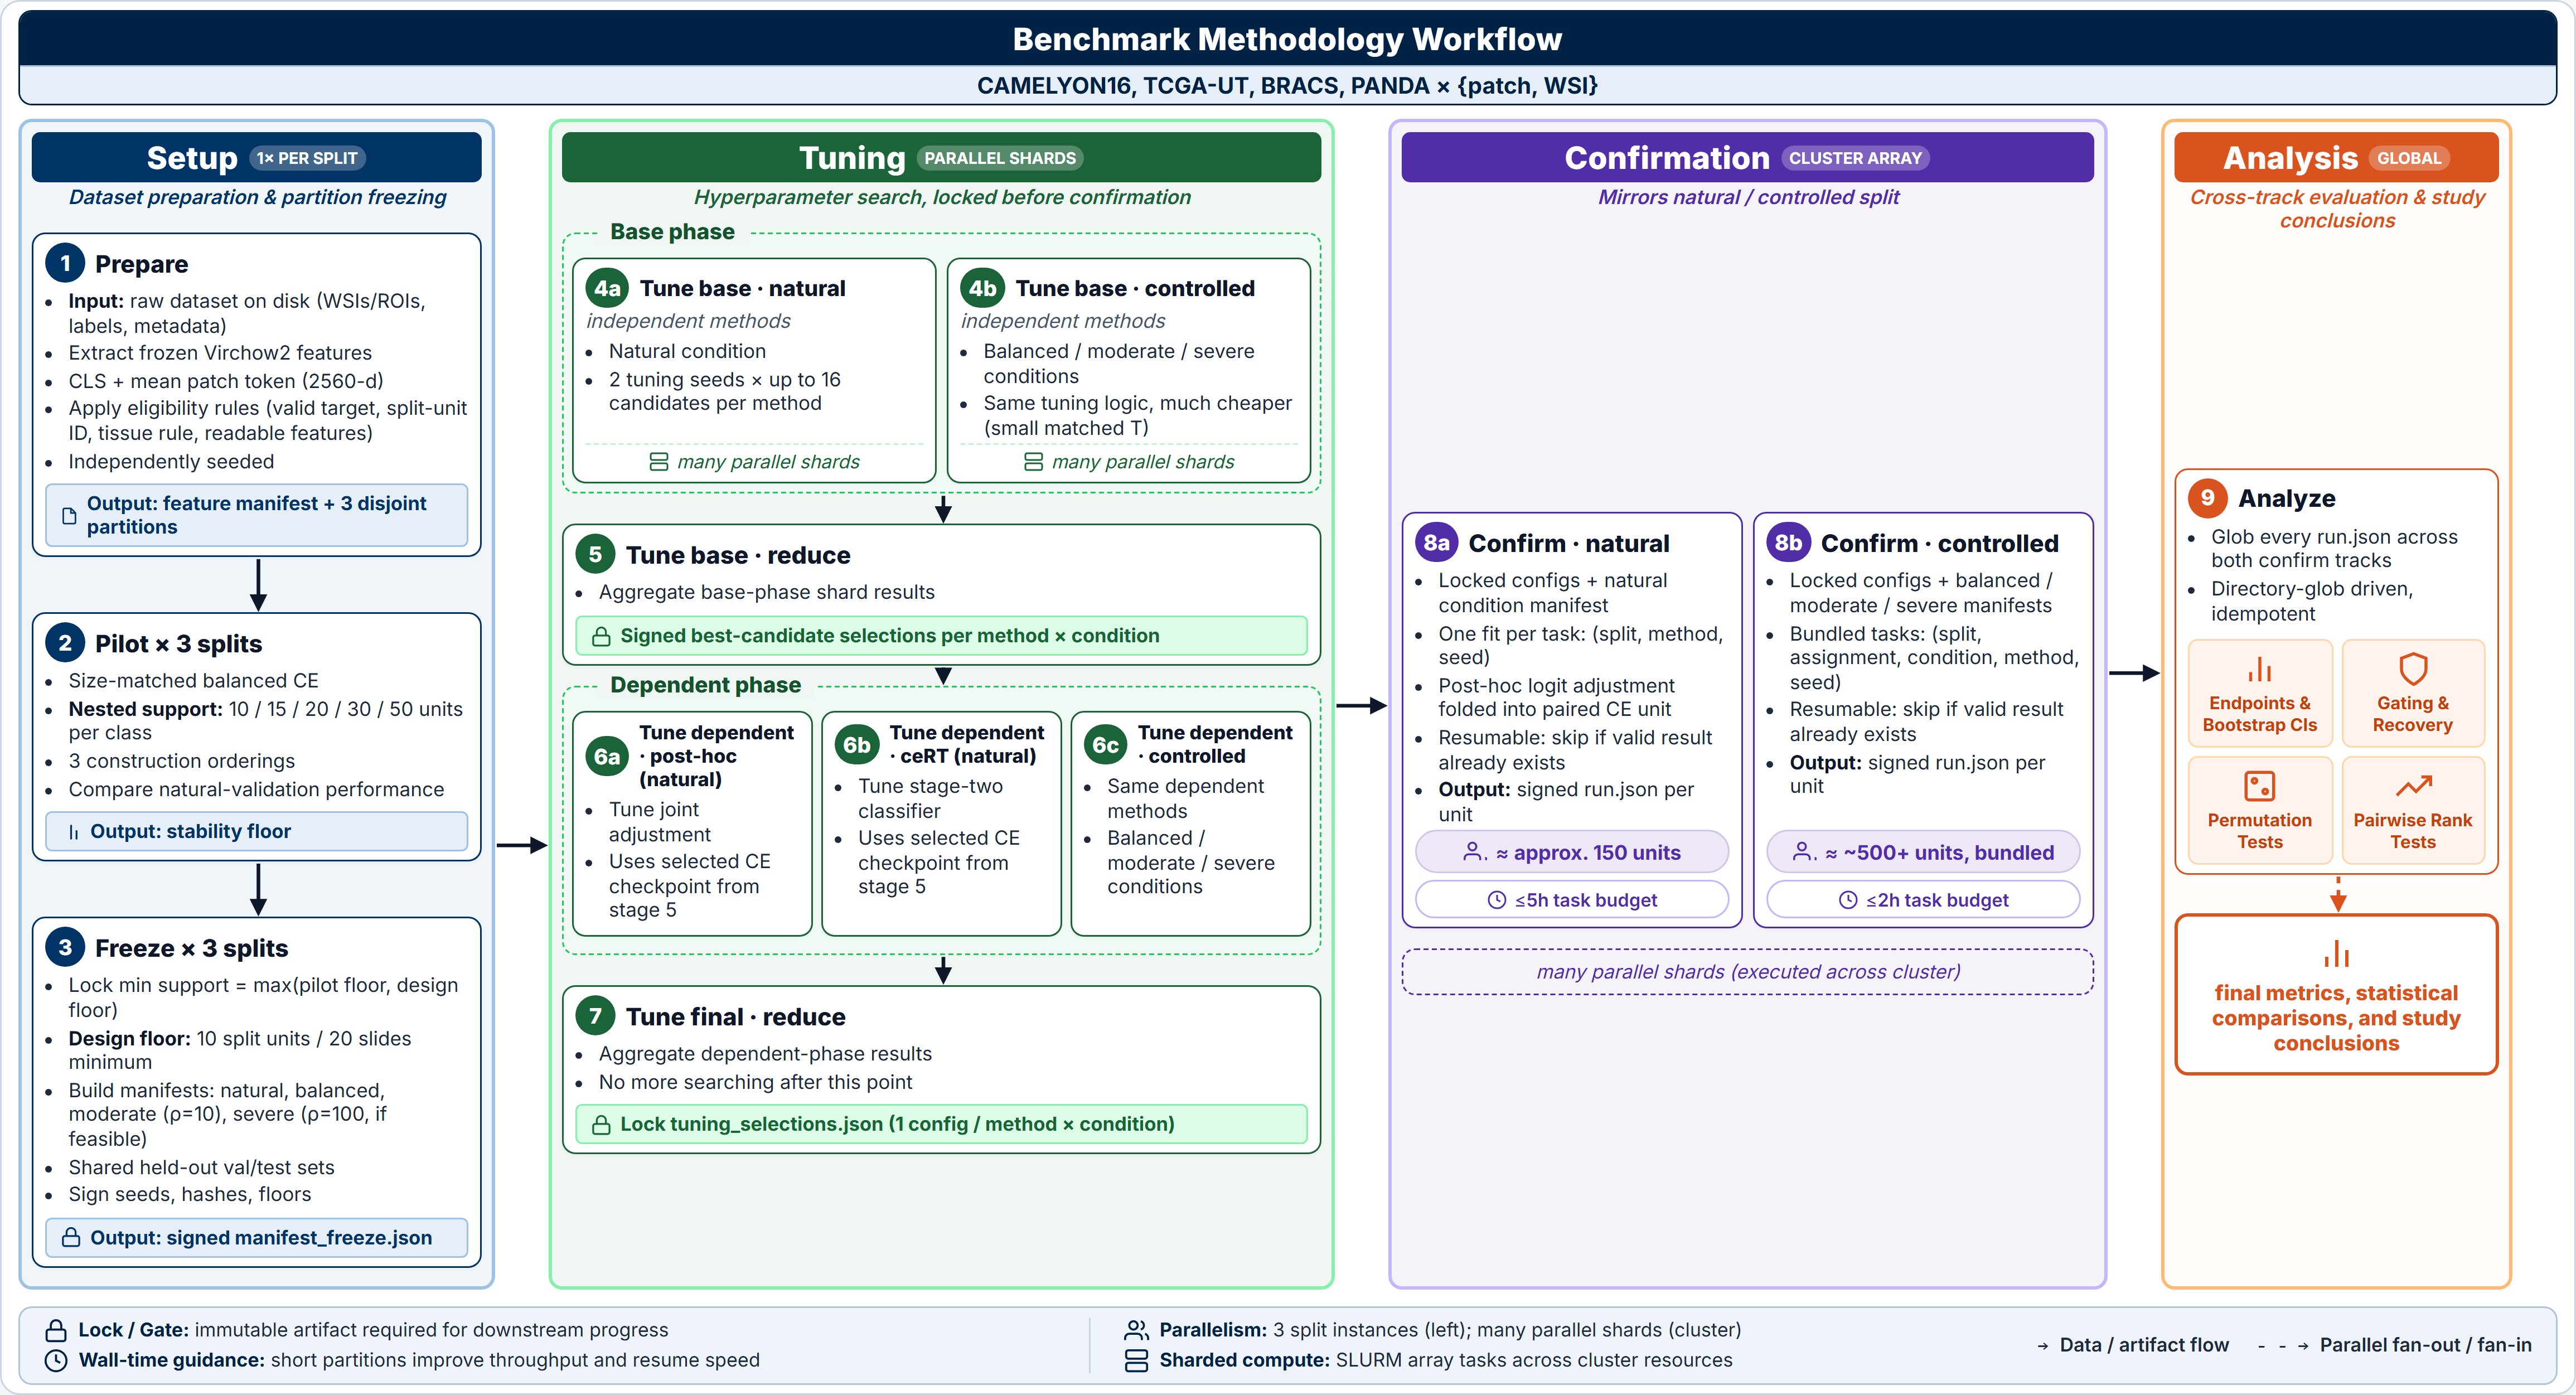
\includegraphics[width=\linewidth,keepaspectratio]{assets/cls_imb_benchmark.png}
  \caption{Overview of the controlled class-imbalance benchmark.}
  \label{fig:benchmark-overview}
\end{figure}
\end{landscape}

\section{Experimental Controls}
\label{app:controls}
Every trainable method uses the common learning-rate grid
\begin{equation}
  \eta\in\{\num{1e-4},\num{3e-4},\num{1e-3},\num{3e-3}\}.
  \label{eq:learning-rate-grid}
\end{equation}
\noindent For methods in Table~\ref{tab:controls}, this grid is crossed with the four candidate values of the method-specific control. The resulting maximum is 16 configurations per method, dataset, regime, and severity. Any computationally necessary narrowing is completed and recorded in the signed analysis manifest before the first definitive fit; no grid is changed once definitive training begins.

\begin{table}[H]
  \centering
  \footnotesize
  \begin{tabularx}{\linewidth}{@{}lX@{}}
    \toprule
    Method or family & Candidate method-specific control \\
    \midrule
    Balanced sampling / weighted CE & strength $\in\{0.25,0.5,0.75,1\}$ \\
    Focal loss & $\gamma\in\{0.5,1,1.5,2\}$ \\
    Logit adjustment & $\tau\in\{0.25,0.5,1,2\}$ \\
    CE + soft F1 / soft MCC & auxiliary weight $\in\{0.25,1,4,16\}$ \\
    CFAL & affinity bandwidth $\sigma\in\{0.25,1,2,4\}$ \\
    OKO & odd-class count $k\in\{1,2,4,8\}$, capped by $K-1$ \\
    RankMix-inspired & beta shape $\alpha\in\{0.5,1,2,4\}$ \\
    SC-MIL & temperature $\tau\in\{0.05,0.1,0.5,1\}$ \\
    MDE-inspired & consistency weight $\lambda_{\mathrm{con}}\in\{0,0.1,0.25,0.5\}$ \\
    \bottomrule
  \end{tabularx}
  \caption{Prespecified method-specific grids crossed with the common learning-rate grid in Equation~\eqref{eq:learning-rate-grid}. cRT has no imbalance-strength grid; only its stage-two learning rate is selected separately.}
  \label{tab:controls}
\end{table}

For every realized condition, the experiment record contains dataset version; eligibility rules; split-unit, slide, and patch identifiers by partition; requested and achieved $T$ and $\rho$; class assignment; all seed families and their tuning, confirmation, pilot, or definitive roles; pilot patch quota; bootstrap-preflight diagnostics; model and optimizer configuration; candidate grid; selected checkpoint; environment identifier; and test-prediction hash. Deviations are dated and justified before the affected test labels are accessed.

\section{Terminology}
\begin{description}
  \item[Natural anchor.] The full eligible natural training partition. It is descriptive and may have a different size from controlled conditions.
  \item[Size-matched balanced reference.] A training subset with total support $T$ and approximately equal class counts; it defines the counterfactual reference in $D_M$.
  \item[Imbalance severity.] The requested training allocation summarized by $\rho$; achieved severity is computed from realized integer counts.
  \item[Pilot level.] A candidate number of independent training units per class used in the balanced CE support-stability study.
  \item[Tail assignment.] The locked mapping from semantic classes to positions in the constructed support profile.
  \item[Comparison unit.] One dataset, prediction regime, imbalance severity, and tail assignment evaluated together.
  \item[Deficit gate.] A prespecified threshold rule that determines whether an observed discrimination or calibration deficit is large and precise enough for recovery analysis.
  \item[Imbalance deficit.] The paired balanced-CE minus imbalanced-CE difference at common $T$ and on the same held-out cases.
  \item[Recovery.] A method's improvement over imbalanced CE divided by the evidenced imbalance deficit.
  \item[Kish effective split-unit count.] The equally weighted split-unit count with the same weight concentration as one bootstrap replicate.
  \item[Intraclass correlation.] The estimated similarity of class margins from patches belonging to the same split-unit or slide cluster.
  \item[Patch-micro estimate.] A metric computed over eligible patch predictions, with split-unit-clustered uncertainty.
  \item[Case-macro estimate.] An equal-weight aggregation over slides or split units, limiting domination by heavily tiled cases.
\end{description}

\clearpage
\bibliographystyle{plainnat}
\bibliography{references}

\end{document}
